\documentclass[12pt,a4paper]{article}
\usepackage[utf8]{inputenc}
\usepackage[english]{babel}
\usepackage{amsmath}
\usepackage{amsfonts}
\usepackage{amssymb}
\usepackage{graphicx}
\usepackage{geometry}
\usepackage{float}
\usepackage{listings}
\usepackage{xcolor}
\usepackage{booktabs}
\usepackage{caption}
\usepackage{subcaption}
\usepackage{fancyhdr}
\usepackage[hidelinks]{hyperref}
\geometry{margin=1in}
\pagestyle{fancy}
\fancyhf{}
\fancyhead[L]{UEFA Euro 2024 Analytics Dashboard}
\fancyhead[R]{\thepage}

\begin{document}

% Custom title page
\begin{titlepage}
    \centering
    
    % University logo space (if available)
    \vspace*{1cm}
    
    %The visualizations presented in this appendix demonstrate the practical implementation of the theoretical frameworks discussed throughout this document:

    {\Large \textbf{HOCHSCHULE FULDA} \par}
    {\large \textbf{UNIVERSITY OF APPLIED SCIENCES} \par}
    \vspace{0.5cm}
    
    % Department
    {\large DEPARTMENT OF APPLIED COMPUTER SCIENCE \par}
    {\large MASTER OF SCIENCE DATA SCIENCE \par}
    \vspace{2cm}
    
    % Course information
    {\Large \textbf{Data Visualization} \par}
    {\large Course Code: AI5170 \par}
    \vspace{2cm}
    
    % Project title
    {\Huge \textbf{UEFA Euro 2024 Analytics Dashboard} \par}
    \vspace{0.5cm}
    {\LARGE \textbf{A Comprehensive Football Data Visualization Platform} \par}
    \vspace{3cm}
    
    % Student information
    {\large \textbf{Submitted by:} \par}
    \vspace{0.5cm}
    
    \begin{tabular}{l}
        \textbf{Muhammad Abdullah Hayat} \\
        Student ID: fd0002018 \\
        Email: muhammad-abdullah.hayat@informatik.hs-fulda.de \\
        \\
        \textbf{Muhammad Khurram Meraj} \\
        Student ID: fd0002044 \\
        Email: muhammad-khurram.meraj@informatik.hs-fulda.de \\
    \end{tabular}
    
    \vfill
    
    % Date
    {\large \today \par}
    
\end{titlepage}

\tableofcontents
\newpage

\section{Overview}

This document presents a comprehensive technical analysis of the UEFA Euro 2024 Analytics Dashboard, an advanced football data visualization platform built using Python's Dash framework and StatsBomb's open football dataset. The system provides interactive analysis capabilities for tournament-wide statistics, detailed match breakdowns, individual player performance metrics, tactical formations, and raw event data exploration.

The dashboard employs a sophisticated dual visualization approach, combining Plotly's interactive web-based charts with Matplotlib's specialized football visualizations through the mplsoccer library. This hybrid strategy maximizes analytical depth while maintaining user accessibility across different levels of football expertise.

Key achievements include implementation of real-time data filtering, multi-dimensional performance analysis, tactical pattern recognition, and professional-grade sports visualization following established football analytics conventions. The system demonstrates robust data engineering practices with intelligent caching strategies, efficient coordinate transformation algorithms, and scalable component architecture.

\section{Introduction and Project Overview}

\subsection{Project Motivation}

Football analytics has evolved significantly in recent years, with data-driven insights becoming crucial for tactical understanding, player evaluation, and strategic decision-making. The UEFA Euro 2024 tournament provided an excellent opportunity to develop a comprehensive analytics platform that bridges the gap between raw event data and actionable insights.

The primary motivation was to create an accessible yet sophisticated tool that enables different stakeholders from casual fans to tactical analysts to explore football data through intuitive visualizations while maintaining analytical rigor.

\subsection{System Objectives}

The dashboard was designed with four core objectives:
\begin{enumerate}
    \item \textbf{Accessibility}: Provide intuitive interfaces for users with varying levels of football analytics expertise
    \item \textbf{Comprehensiveness}: Cover all aspects of football analysis from individual events to tournament-wide patterns
    \item \textbf{Interactivity}: Enable dynamic data exploration through filtering, selection, and drill-down capabilities
    \item \textbf{Professional Quality}: Implement visualization standards that meet professional sports analytics requirements
\end{enumerate}

\subsection{Technical Foundation}

The system is built on StatsBomb's open football dataset, which provides event-level data for all UEFA Euro 2024 matches. This dataset includes detailed spatial and temporal information for every action during matches, from passes and shots to defensive actions and set pieces.

\section{Data Sources and Acquisition}

\subsection{StatsBomb Dataset Overview}

The foundation of our analytics platform is StatsBomb's comprehensive UEFA Euro 2024 dataset\footnote{See: \url{https://github.com/statsbomb/open-data}}, accessed through their official Python API (\texttt{statsbombpy}\footnote{See: \url{https://github.com/statsbomb/statsbombpy}}). This dataset represents one of the most detailed publicly available football datasets, containing event-level information for all tournament matches.

\paragraph{Dataset Characteristics:}
\begin{itemize}
    \item \textbf{Competition}: UEFA Euro 2024 (Competition ID: 55, Season ID: 282)
    \item \textbf{Coverage}: Complete tournament data including all 51 matches
    \item \textbf{Granularity}: Event-level data with millisecond timestamp precision
    \item \textbf{Spatial Resolution}: Coordinate data with 120x80 pitch dimension normalization
    \item \textbf{Data Volume}: Approximately 45,000+ events per match
\end{itemize}

\section{Visualization Design and Implementation}
\label{sec:visualization_design}

\subsection{Tournament Overview Dashboard}

The tournament overview component provides high-level tournament statistics and insights through an intuitive header with key metrics and three main analysis tabs. While traditional EDA (Explorative Data Analysis) often begins with univariate and bivariate statistics, our dataset comprising event timelines from football matches necessitated a top-down approach. Therefore, we started with a tournament overview and progressively drilled down to match-level and player-level insights, ensuring comprehensive coverage from the broadest patterns to the most granular details.


\subsubsection{Key Stats}
\begin{itemize}
    \item \textbf{Match Counting}: Aggregates total matches from the competition dataset
    \item \textbf{Goal Summation}: Sums goals across all matches in the tournament
    \item \textbf{Team Extraction}: Identifies unique teams participating in the competition
    \item \textbf{Average Calculation}: Computes goals per match ratio with single decimal precision
\end{itemize}

Rather than using raw API data, these statistics are pre-calculated and cached to improve performance and ensure consistency across dashboard components.

\subsubsection{Goals Analysis Tab}
This tab presents a comprehensive horizontal bar chart ranking teams by total goals scored throughout the tournament. The visualization employs color intensity mapping where deeper blue shades indicate higher-scoring teams, creating immediate visual identification of offensive prowess. The chart includes hover functionality revealing goals per match ratios for efficiency analysis.


\subsubsection{Team Performance Tab}
Features dual visualizations: a comprehensive standings table with color-coded metrics and a stacked horizontal bar chart showing win/draw/loss percentages for top teams. The table uses semantic colors (green for positive outcomes, red for negative) while the bar chart reveals performance consistency patterns. Figure \ref{fig:team_comparison} in Appendix A demonstrates the practical implementation of this comprehensive team analysis approach.


\subsubsection{Match Insights Tab}
Presents tournament-wide statistical patterns through histograms showing goals per match distribution and goal difference distribution, complemented by a pie chart breaking down match outcomes. This multi-visualization approach exposes competitive balance and scoring trends.



\subsection{Match Overview Dashboard}
\label{sec:match_overview}

The match overview component provides comprehensive match analysis through a hierarchical layout with team/match selection and six coordinated visualization tabs. 

\subsubsection{Shot Maps with Expected Goals (xG) Visualization}
\label{sec:shot_maps}
Shot maps employ spatial positioning combined with size encoding to represent shot quality:
\begin{itemize}
    \item \textbf{Spatial Encoding}: Shot locations on accurate football pitch representation using mplsoccer coordinates
    \item \textbf{Size Encoding}: Circle size proportional to xG value for immediate quality assessment
    \item \textbf{Color Encoding}: Distinct colors for goals versus other shot outcomes (goals in red, shots in blue)
    \item \textbf{Interactive Features}: Hover details with xG values, and shot outcome
\end{itemize}

Figure \ref{fig:shot_map} demonstrates the practical implementation of this shot visualization methodology.

\subsubsection{Pass Network Analysis}
\label{sec:pass_network}
Pass networks utilize force-directed graph layouts combined with spatial positioning to reveal team structure and player relationships:
\begin{itemize}
    \item \textbf{Node Size}: Proportional to passing involvement (total passes + receptions)
    \item \textbf{Edge Thickness}: Pass frequency between specific player pairs
    \item \textbf{Spatial Layout}: Average field positions determine node placement
    \item \textbf{Label Strategy}: Position acronyms for tactical clarity over player names
\end{itemize}

A detailed example of this network analysis implementation is shown in Figure \ref{fig:pass_network}, demonstrating the Spain vs England passing relationships during their UEFA Euro 2024 encounter.



\subsubsection{Expected Goals Timeline}
xG progression visualization uses cumulative line charts with event annotations to show match momentum:
\begin{itemize}
    \item \textbf{Cumulative Approach}: Running xG totals show momentum shifts throughout match duration
    \item \textbf{Goal Annotations}: Vertical lines marking actual goals for xG vs reality comparison
    \item \textbf{Team Comparison}: Dual lines enable direct performance comparison between teams
    \item \textbf{Interactive Exploration}: Hover details reveal specific time periods and xG contributions
\end{itemize}



\subsubsection{Match Statistics Tab}
\label{sec:match_statistics}
Comprehensive side-by-side team comparison using symmetric horizontal bar charts:
\begin{itemize}
    \item \textbf{Symmetric Layout}: Teams displayed on opposite sides for direct comparison
    \item \textbf{Metric Categorization}: Statistics grouped by type (possession, shooting, passing, defensive)
    \item \textbf{Value Encoding}: Bar length proportional to metric values with team colors
    \item \textbf{Percentage Display}: Key metrics shown as percentages for standardized comparison
\end{itemize}

\subsubsection{Key Events Timeline Tab}
Chronological visualization of significant match events with color-coded team identification:
\begin{itemize}
    \item \textbf{Event Filtering}: Goals, cards, substitutions extracted from full event stream
    \item \textbf{Temporal Layout}: Events positioned by match minute on horizontal timeline
    \item \textbf{Color Coding}: Team colors distinguish event ownership
    \item \textbf{Event Details}: Player names, event types, and contextual information displayed
\end{itemize}

\subsubsection{Formations Analysis Tab}
\label{sec:formations_analysis}
Team formation visualization using mplsoccer with individual player activity density plots:
\begin{itemize}
    \item \textbf{Formation Grid Layout}: Individual subplots for each player position using mplsoccer's formation grid system
    \item \textbf{Activity Density Visualization}: KDE plots showing player movement patterns based on Ball Receipt events
    \item \textbf{Formation Recognition}: Tactical setup identified and labeled from Starting XI data
    \item \textbf{Position Offset Application}: Predefined formation-specific offsets prevent overlapping position displays
\end{itemize}

The practical implementation of this formation analysis is illustrated in Figure \ref{fig:formations}, showing the tactical positioning and formation structure visualization.


\subsection{Player Performance Dashboard}
\label{sec:player_performance}

The player performance dashboard provides individual player analysis through a hierarchical selection interface and four specialized visualization tabs.


\subsubsection{Player Data Processing and Aggregation}
The dashboard performs extensive data manipulation to extract player-specific insights:

\subsubsection{Shot Analysis Tab}
Displays player-specific shot maps using matplotlib with precise spatial positioning on football pitches:
\begin{itemize}
    \item \textbf{Spatial Accuracy}: Shot locations plotted using mplsoccer coordinate system
    \item \textbf{Quality Encoding}: Circle sizes proportional to xG values for immediate quality assessment
    \item \textbf{Outcome Differentiation}: Goals marked with distinct football icons, shots with circles
    \item \textbf{Context Information}: Hover details include shot context, time, and opponent
\end{itemize}



\subsubsection{Touch Heatmap Tab}
\label{sec:touch_heatmap}
Employs binned spatial analysis using a 6x5 grid system rather than continuous density estimation:
\begin{itemize}
    \item \textbf{Grid-Based Analysis}: 30 standardized zones providing interpretable spatial regions
    \item \textbf{Percentage Quantification}: Activity distribution calculated and labeled numerically
    \item \textbf{Color Intensity Mapping}: White-to-red gradient indicating activity frequency
    \item \textbf{Cross-Player Standardization}: Consistent binning enables direct player comparisons
\end{itemize}

Figure \ref{fig:touch_heatmap} demonstrates this grid-based approach, showing how player activity is distributed across standardized pitch zones with percentage-based quantification.


\subsubsection{Progressive Actions Tab}
Analyzes forward ball progression through horizontal bar charts showing progressive passes by team context:
\begin{itemize}
    \item \textbf{Definition Clarity}: Progressive passes defined as movements advancing ball greater than 10 meters toward opponent's goal
    \item \textbf{Team Context Provision}: Selected player highlighted within team ranking
    \item \textbf{Ranking Visualization}: Horizontal bars enable clear comparison across team members
    \item \textbf{Contextual Information}: Additional metrics like total passes and success rates included
\end{itemize}


\subsubsection{Performance Metrics Tab}
\label{sec:performance_metrics}
Introduces innovative dual radar chart methodology separating volume and success rate metrics:
\begin{itemize}
    \item \textbf{Volume Radar}: Goals, shots, passes, dribbles, duels, interceptions (normalized to 0-100 scale)
    \item \textbf{Success Rate Radar}: Pass accuracy, dribble success, shot accuracy, duel success rates (0-100\% scale)
    \item \textbf{Color Distinction}: Blue for volume metrics, green for success rates preventing conflation
    \item \textbf{Multi-Player Overlay}: Comparison player data overlaid for direct performance comparison
\end{itemize}

The implementation of this dual radar chart innovation is showcased in Figure \ref{fig:player_performance}, demonstrating how volume and success rate metrics are effectively separated to prevent analytical confusion.



\subsection{Tactical Analysis Component}
\label{sec:tactical_analysis}

The tactical analysis component focuses on team-level patterns and strategic insights through a hierarchical selection interface and four specialized analysis types.

\subsubsection{Formation Analysis Tab}
\label{sec:tactical_formation}
Displays team shape and player positioning through comprehensive formation visualization:
\begin{itemize}
    \item \textbf{Average Position Calculation}: Player positions computed from first 15 minutes of match data
    \item \textbf{Position Offset System}: Overlapping positions separated using formation-specific offset algorithms
    \item \textbf{Role Color Coding}: Players color-coded by position type (defenders, midfielders, forwards)
    \item \textbf{Tactical Context}: Formation name and tactical description provided
\end{itemize}



\subsubsection{Defensive Actions Tab}
Explores defensive coverage and tactics through spatial analysis of defensive events:
\begin{itemize}
    \item \textbf{Action Type Coverage}: Tackles, interceptions, blocks, and clearances mapped spatially
    \item \textbf{Density Heat mapping}: Defensive activity intensity shown across pitch zones
    \item \textbf{Success Rate Overlays}: Defensive action effectiveness integrated with spatial data
    \item \textbf{Pressure Zones}: Areas of high defensive pressure identified and highlighted
\end{itemize}



\subsubsection{Attacking Patterns Tab}
Examines offensive strategies in the final third through comprehensive attacking action analysis:
\begin{itemize}
    \item \textbf{Final Third Focus}: Events filtered to attacking third of the pitch (x > 80)
    \item \textbf{Action Type Analysis}: Shots, dribbles, key passes, and crosses analyzed spatially
    \item \textbf{Creation Zones}: Areas of attack initiation and completion mapped
    \item \textbf{Success Rate Integration}: Attacking effectiveness calculated by zone and action type
\end{itemize}


\subsubsection{Set Pieces Tab}
Analyzes corners, free kicks, and throw-ins through comprehensive set piece evaluation:
\begin{itemize}
    \item \textbf{Set Piece Classification}: Events categorized by type (corner, free kick, throw-in)
    \item \textbf{Frequency Analysis}: Set piece counts and success rates calculated
    \item \textbf{Spatial Distribution}: Set piece locations and outcomes mapped
    \item \textbf{Effectiveness Metrics}: Goals and chances created from set pieces analyzed
\end{itemize}


\subsubsection{Detailed Analysis Components}
The dashboard includes two secondary visualizations providing complementary insights:
\begin{itemize}
    \item \textbf{Pass Length Distribution}: Histogram showing team passing patterns and preferences
    \item \textbf{Event Timeline}: Match minute activity distribution revealing tactical periods
\end{itemize}

\subsubsection{Team Comparison Visualization}
Symmetric horizontal bar charts enable immediate tactical comparison between both teams:
\begin{itemize}
    \item \textbf{Symmetric Layout}: Teams displayed on opposite sides for direct comparison
    \item \textbf{Metric Categorization}: Tactical statistics grouped by type (passing, attacking, defensive)
    \item \textbf{Normalized Scaling}: Metrics scaled appropriately for fair comparison across different measurement units
    \item \textbf{Color Consistency}: Team colors maintained throughout for visual continuity and immediate identification
\end{itemize}


\subsection{Event Explorer Interface}
\label{sec:event_explorer}

The event explorer provides granular access to raw event data through a comprehensive filtering interface and three main visualization tabs with integrated data export capabilities.


\subsubsection{Event Timeline Tab}
Displays temporal event distribution with enhanced analytical capabilities:
\begin{itemize}
    \item \textbf{Frequency Analysis}: Events aggregated by minute showing match intensity patterns
    \item \textbf{Activity Peak Identification}: High-activity periods highlighted for tactical analysis
    \item \textbf{Dynamic Filtering Integration}: Timeline updates in real-time based on all applied filters
    \item \textbf{Interactive Exploration}: Hover functionality reveals detailed event breakdowns
\end{itemize}


\subsubsection{Event Heatmap Tab}
\label{sec:event_heatmap}
Combines spatial accuracy with statistical insights through football pitch-based density visualization:
\begin{itemize}
    \item \textbf{Spatial Event Density}: Event concentration mapped to accurate football pitch coordinates
    \item \textbf{Pitch Context Integration}: mplsoccer library ensures proper spatial representation
    \item \textbf{Density Gradient Encoding}: Color intensity indicates event frequency with darker areas showing higher activity
    \item \textbf{Filter Integration}: Heatmap updates based on event type and player selections
\end{itemize}

Figure \ref{fig:events_heatmap} illustrates this comprehensive spatial analysis approach, showing how all match events are mapped to accurate football pitch coordinates with density-based visualization.



\subsubsection{Event Distribution Tab}
Presents categorical event analysis through team-comparative visualization:
\begin{itemize}
    \item \textbf{Event Type Breakdown}: Nine event categories analyzed with frequency and percentage calculations
    \item \textbf{Team Comparison}: Side-by-side analysis enabling tactical approach identification
    \item \textbf{Category Ranking}: Events sorted by frequency for immediate pattern recognition
    \item \textbf{Filter Responsiveness}: Distribution updates based on all applied filtering criteria
\end{itemize}


\subsubsection{Interactive Data Table with Export Capabilities}
Comprehensive tabular interface providing detailed event examination:
\begin{itemize}
    \item \textbf{Dynamic Column Display}: Table columns adapt based on available event data fields
    \item \textbf{Native Filtering}: Built-in search and filter functionality for each column
    \item \textbf{Pagination System}: 20 events per page with navigation controls
    \item \textbf{Export Functionality}: CSV download maintaining all applied filters
\end{itemize}


\subsubsection{Summary Statistics Integration}
Dynamic summary panel providing filtered dataset context:
\begin{itemize}
    \item \textbf{Event Count}: Total events in filtered dataset
    \item \textbf{Player Involvement}: Number of unique players in filtered events
    \item \textbf{Dominant Event Type}: Most frequent event category with percentage
    \item \textbf{Temporal Window}: Active time range for filtered data
\end{itemize}




\section{Visualization Design Philosophy and Approach Selection}
\label{sec:design_philosophy}

This section consolidates the design rationale and alternative approaches considered for each dashboard component, providing comprehensive insight into the visualization selection methodology employed throughout the analytics platform.

\subsection{Tournament Overview Dashboard Design Decisions}

\subsubsection{Goals Analysis Horizontal Bar Charts}
\textbf{Alternative Visualizations Considered:}
\begin{itemize}
    \item \textbf{Scatter plots}: Goals vs matches could show efficiency trends but would lose the clear hierarchical ranking and immediate comparison capability
    \item \textbf{Heat maps}: Would emphasize extremes but sacrifice readability for team names and precise values
    \item \textbf{Radar charts}: Could show multiple metrics simultaneously but would complicate the primary goals focus and reduce comparison clarity
    \item \textbf{Bubble charts}: Size and position encoding would be less precise than horizontal bars for ranking visualization
\end{itemize}

\textbf{Design Decision Rationale:}
Horizontal bar charts were chosen because they excel at ranking visualization, support team name labels effectively, and enable precise value comparison. The horizontal orientation accommodates longer team names better than vertical bars.

\subsubsection{Team Performance Dual Visualization Approach}
\textbf{Alternative Approaches Considered:}
\begin{itemize}
    \item \textbf{Single table view}: Would be more compact but lose the visual impact of percentage distributions
    \item \textbf{Pie charts for each team}: Individual pies would be comprehensive but difficult to compare across teams
    \item \textbf{Line graphs}: Better for trends over time but tournament format has limited temporal progression
\end{itemize}

\textbf{Design Decision Rationale:}
The dual visualization approach combines the precision of tabular data with the visual impact of percentage distributions. Stacked bars enable immediate comparison of team consistency and performance patterns.

\subsubsection{Match Insights Statistical Presentations}
\textbf{Alternative Statistical Presentations:}
\begin{itemize}
    \item \textbf{Box plots}: Would show quartiles and outliers but be less accessible to general audiences
    \item \textbf{Violin plots}: Kernel density estimation would be more sophisticated but harder to interpret
    \item \textbf{Summary statistics table}: More precise but less visually engaging for pattern recognition
\end{itemize}

\textbf{Design Decision Rationale:}
Histograms were chosen for their accessibility and clear pattern revelation. The combination with pie charts provides both distributional understanding and categorical breakdown, serving users with different analytical preferences.

\subsection{Match Overview Dashboard Design Decisions}

\subsubsection{Shot Maps with Expected Goals Visualization}
\textbf{Alternative Approaches Considered:}
\begin{itemize}
    \item \textbf{Heat maps}: Would show shot density patterns but lose individual shot precision and xG values
    \item \textbf{Hexbin plots}: Better for high-density data but Euro 2024 matches have manageable shot counts
    \item \textbf{Contour plots}: Continuous density estimation would be statistically sophisticated but less interpretable
\end{itemize}

\textbf{Design Decision Rationale:}
Scatter plots preserve shot-level granularity essential for tactical analysis while enabling pattern recognition through spatial clustering. Size encoding for xG provides immediate quality assessment without requiring additional visual channels.

\subsubsection{Pass Network Analysis with Force-Directed Layouts}
\textbf{Alternative Network Approaches:}
\begin{itemize}
    \item \textbf{Adjacency matrices}: Precise numerical representation but loses spatial football context
    \item \textbf{Chord diagrams}: Effective for showing relationships but lacks positional information
    \item \textbf{Sankey diagrams}: Good for flow visualization but inappropriate for bidirectional passing
\end{itemize}

\textbf{Design Decision Rationale:}
Network graphs with spatial positioning preserve football-specific spatial context while revealing tactical patterns. The combination enables identification of key players, passing triangles, and formation structure simultaneously.

\subsubsection{Expected Goals Timeline Progression}
\textbf{Alternative Timeline Approaches:}
\begin{itemize}
    \item \textbf{Area charts}: Would emphasize cumulative totals but reduce focus on momentum progression
    \item \textbf{Bar charts by period}: Clearer for period-specific analysis but lose continuous flow narrative
    \item \textbf{Step functions}: More mathematically precise but less visually smooth for general audiences
\end{itemize}

\textbf{Design Decision Rationale:}
Line charts effectively communicate momentum changes and enable easy comparison between teams. Cumulative approach shows match narrative progression better than instantaneous values.

\subsection{Player Performance Dashboard Design Decisions}

\subsubsection{Player Shot Analysis Visualization}
\textbf{Design Decision Rationale:}
The shot map visualization approach mirrors the match overview methodology (see Section~\ref{sec:shot_maps}) but with player-specific filtering and context. This consistency ensures users can seamlessly transition between team-level and individual-level analysis while maintaining spatial accuracy through mplsoccer integration.

\subsubsection{Touch Heatmap Grid-Based Analysis}
\textbf{Alternative Heatmap Approaches:}
\begin{itemize}
    \item \textbf{Continuous density estimation}: Kernel density would show smoother patterns but sacrifice quantifiability
    \item \textbf{Hexagonal binning}: Better for high-density data but less intuitive for football pitch zones
    \item \textbf{Voronoi diagrams}: Mathematically elegant but inappropriate for rectangular pitch analysis
\end{itemize}

\textbf{Design Decision Rationale:}
Grid-based approach balances visual appeal with analytical precision, enabling both qualitative pattern recognition and quantitative comparison across players and positions. The 6x5 grid system provides interpretable spatial regions while maintaining cross-player standardization.

\subsubsection{Progressive Actions Analysis}
\textbf{Alternative Progressive Analysis Approaches:}
\begin{itemize}
    \item \textbf{Network-based analysis}: Pass networks could show progressive connections but lose individual contribution clarity
    \item \textbf{Spatial progression maps}: Field plots could show progression paths but be cluttered for team-wide analysis
    \item \textbf{Time-series analysis}: Temporal progression patterns could be interesting but beyond current scope
\end{itemize}

\textbf{Design Decision Rationale:}
Horizontal bar charts enable clear ranking visualization within team context while maintaining focus on individual contribution metrics. The approach provides immediate comparison capability essential for player evaluation.

\subsubsection{Dual Radar Chart Innovation}
\textbf{Alternative Performance Analysis Approaches:}
\begin{itemize}
    \item \textbf{Combined radar charts}: Single charts would mask critical distinction between activity and effectiveness
    \item \textbf{Parallel coordinates}: Multi-dimensional plots less intuitive for cyclical sports performance data
    \item \textbf{Scatter plot matrices}: Comprehensive but overwhelming for general audience accessibility
    \item \textbf{Performance scorecards}: Tabular presentation more precise but less visually engaging
\end{itemize}

\textbf{Design Decision Rationale:}
Dual radar chart separation prevents the analytical error of conflating player activity level with effectiveness. This innovation enables identification of high-volume/low-success players versus low-volume/high-success players, crucial for tactical understanding.

\subsection{Tactical Analysis Dashboard Design Decisions}

\subsubsection{Formation Analysis Visualization}
\textbf{Alternative Formation Approaches:}
\begin{itemize}
    \item \textbf{Heat maps}: Would show movement patterns but lose formation structure clarity
    \item \textbf{Animation sequences}: Temporal changes visible but overwhelming for formation analysis
    \item \textbf{3D positioning}: Height dimension irrelevant for football tactical analysis
\end{itemize}

\textbf{Design Decision Rationale:}
Static formation display with offset corrections provides clear tactical understanding while maintaining positional accuracy. Color coding enables immediate position role identification essential for tactical analysis.

\subsubsection{Defensive and Attacking Pattern Analysis}
\textbf{Alternative Spatial Analysis Approaches:}
\begin{itemize}
    \item \textbf{Network analysis}: Could show cooperation patterns but lose crucial spatial context
    \item \textbf{Timeline analysis}: Temporal patterns interesting but secondary to spatial positioning
    \item \textbf{Individual player focus}: Personal stats available but team patterns prioritized
\end{itemize}

\textbf{Design Decision Rationale:}
Spatial heat mapping preserves tactical relevance by maintaining football pitch context while revealing team-level patterns. The approach enables identification of strategic zones and tactical preferences essential for coaching analysis.

\subsection{Event Explorer Dashboard Design Decisions}

\subsubsection{Event Timeline Analysis}
\textbf{Alternative Timeline Approaches:}
\begin{itemize}
    \item \textbf{Bar charts}: Would show discrete periods clearly but lose continuous temporal flow
    \item \textbf{Area charts}: Better for cumulative analysis but timeline focus is on frequency patterns
    \item \textbf{Heat map calendars}: Interesting for multiple matches but single-match focus preferred
\end{itemize}

\textbf{Design Decision Rationale:}
Line charts effectively communicate temporal patterns and enable identification of tactical periods. The continuous representation better reveals match flow compared to discrete visualizations.

\subsubsection{Event Heatmap Spatial Analysis}
\textbf{Design Decision Rationale:}
The spatial density approach mirrors the grid-based methodology established in player heatmaps (see Section~\ref{sec:touch_heatmap}) while adapting to event-level granularity. This consistency ensures analytical coherence across dashboard components.

\subsubsection{Event Distribution Categorical Analysis}
\textbf{Alternative Distribution Approaches:}
\begin{itemize}
    \item \textbf{Pie charts}: Would show proportions clearly but team comparison would be difficult
    \item \textbf{Stacked bars}: Could show team and total simultaneously but individual team patterns less clear
    \item \textbf{Radar charts}: Multi-dimensional comparison possible but less accessible for categorical data
\end{itemize}

\textbf{Design Decision Rationale:}
Side-by-side bar charts enable immediate team comparison while preserving categorical clarity. The approach facilitates tactical pattern identification through direct frequency comparison.

\section{Conclusion}
\subsection{Intended Audience and Applications}

\subsubsection{Educators and Learners}
\begin{itemize}
\item \textbf{Tactical Educators and Students}: Ideal for teaching and learning football tactics through visual, data-driven tools.
\item \textbf{Data Science Instructors and Learners}: Offers a real-world case study for data visualization and sports analytics.
\item \textbf{Aspiring Sports Analysts}: Provides hands-on experience with professional-level analytics tools.
\end{itemize}

\subsubsection{Industry Professionals}
\begin{itemize}
\item \textbf{Coaching and Technical Staff}: Supports match analysis and tactical planning with in-depth visual insights.
\item \textbf{Journalists and Broadcasters}: Enhances storytelling and analysis with engaging and insightful graphics.
\item \textbf{Football Fans and Communities}: Enables data-savvy fans to explore tournament trends and player performances in detail.
\end{itemize}

\subsection{Final Remarks}

This project demonstrates the successful application of modern data science and visualization techniques to the complex domain of football analytics. The combination of robust engineering practices, innovative visualization approaches, and user-centered design principles creates a comprehensive platform that advances the state of the art in sports data visualization.

The modular architecture and careful attention to performance optimization ensure that the system can serve as a foundation for future developments in real-time analytics, machine learning integration, and enhanced user experiences. As football analytics continues to evolve, platforms like this dashboard will play an increasingly important role in translating complex data into actionable insights for coaches, analysts, and fans alike.

The successful completion of this project validates the potential for sophisticated data visualization to democratize access to professional-level sports analytics, making advanced analytical capabilities accessible to broader audiences while maintaining the depth and accuracy required for professional applications.

\newpage
\appendix
\section{Advanced Dashboard Visualizations}

This appendix presents key visualizations generated by the Dashboard, demonstrating the practical implementation of the analytical frameworks discussed throughout this document. Each figure showcases different aspects of the football analytics platform.

\subsection{Match Overview Analysis Visualizations}
\begin{figure}[H]
    \centering
    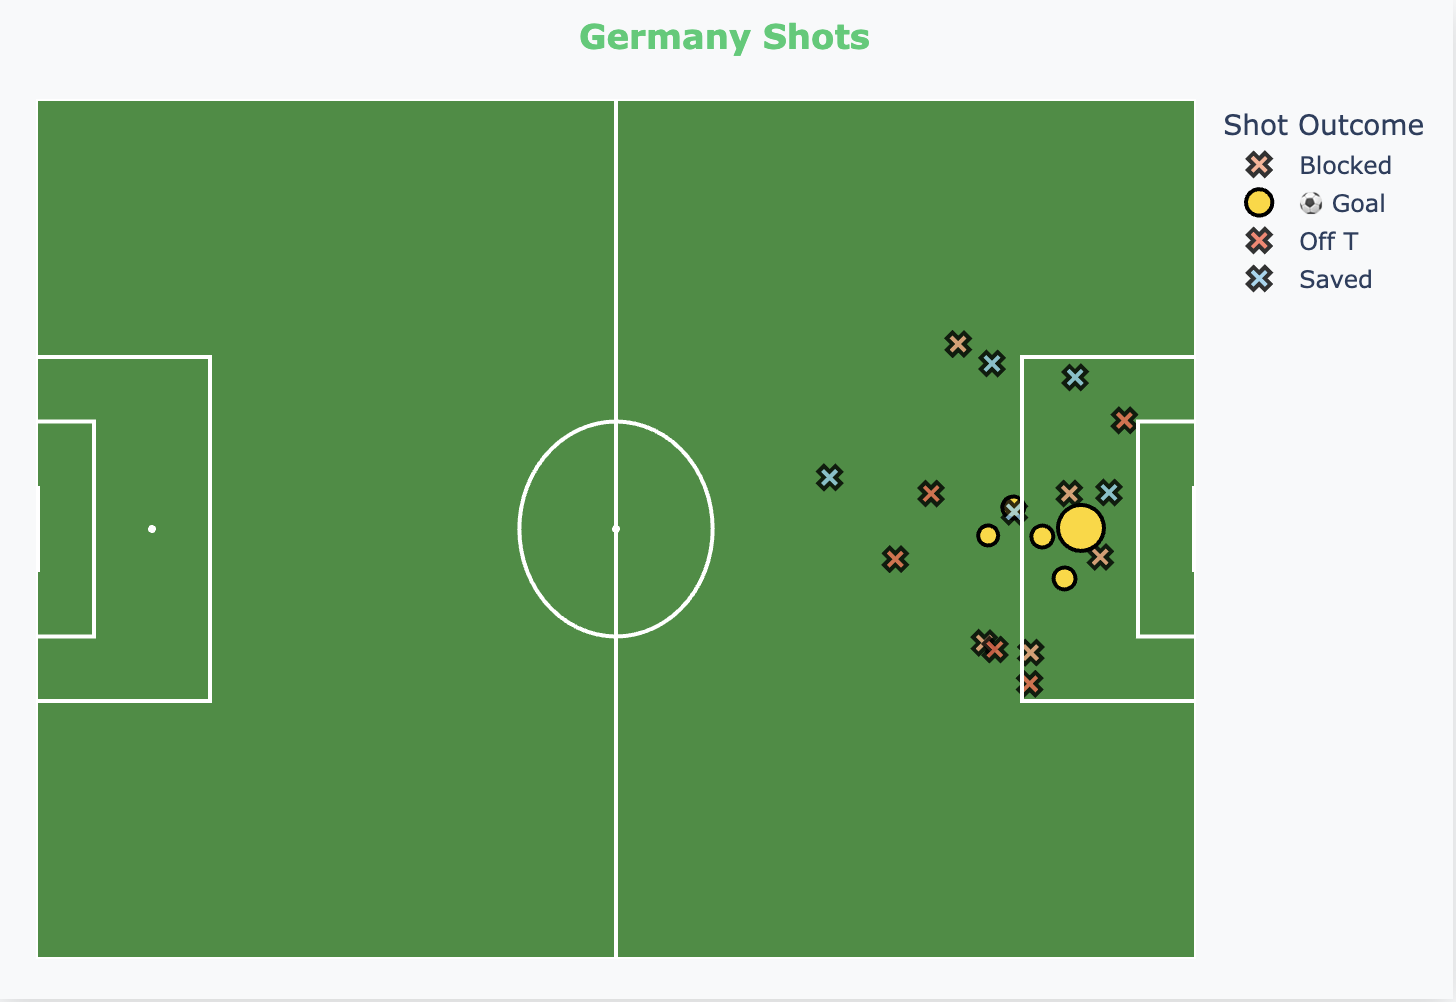
\includegraphics[width=0.85\textwidth]{Shots Map.png}
    \caption{Shot Map Visualization analysis showing shot locations with size encoding proportional to xG values. Goals are distinguished from other shot outcomes through distinct visual markers, as described in Section~\ref{sec:shot_maps}.}
    \label{fig:shot_map}
\end{figure}
\begin{figure}[H]
    \centering
    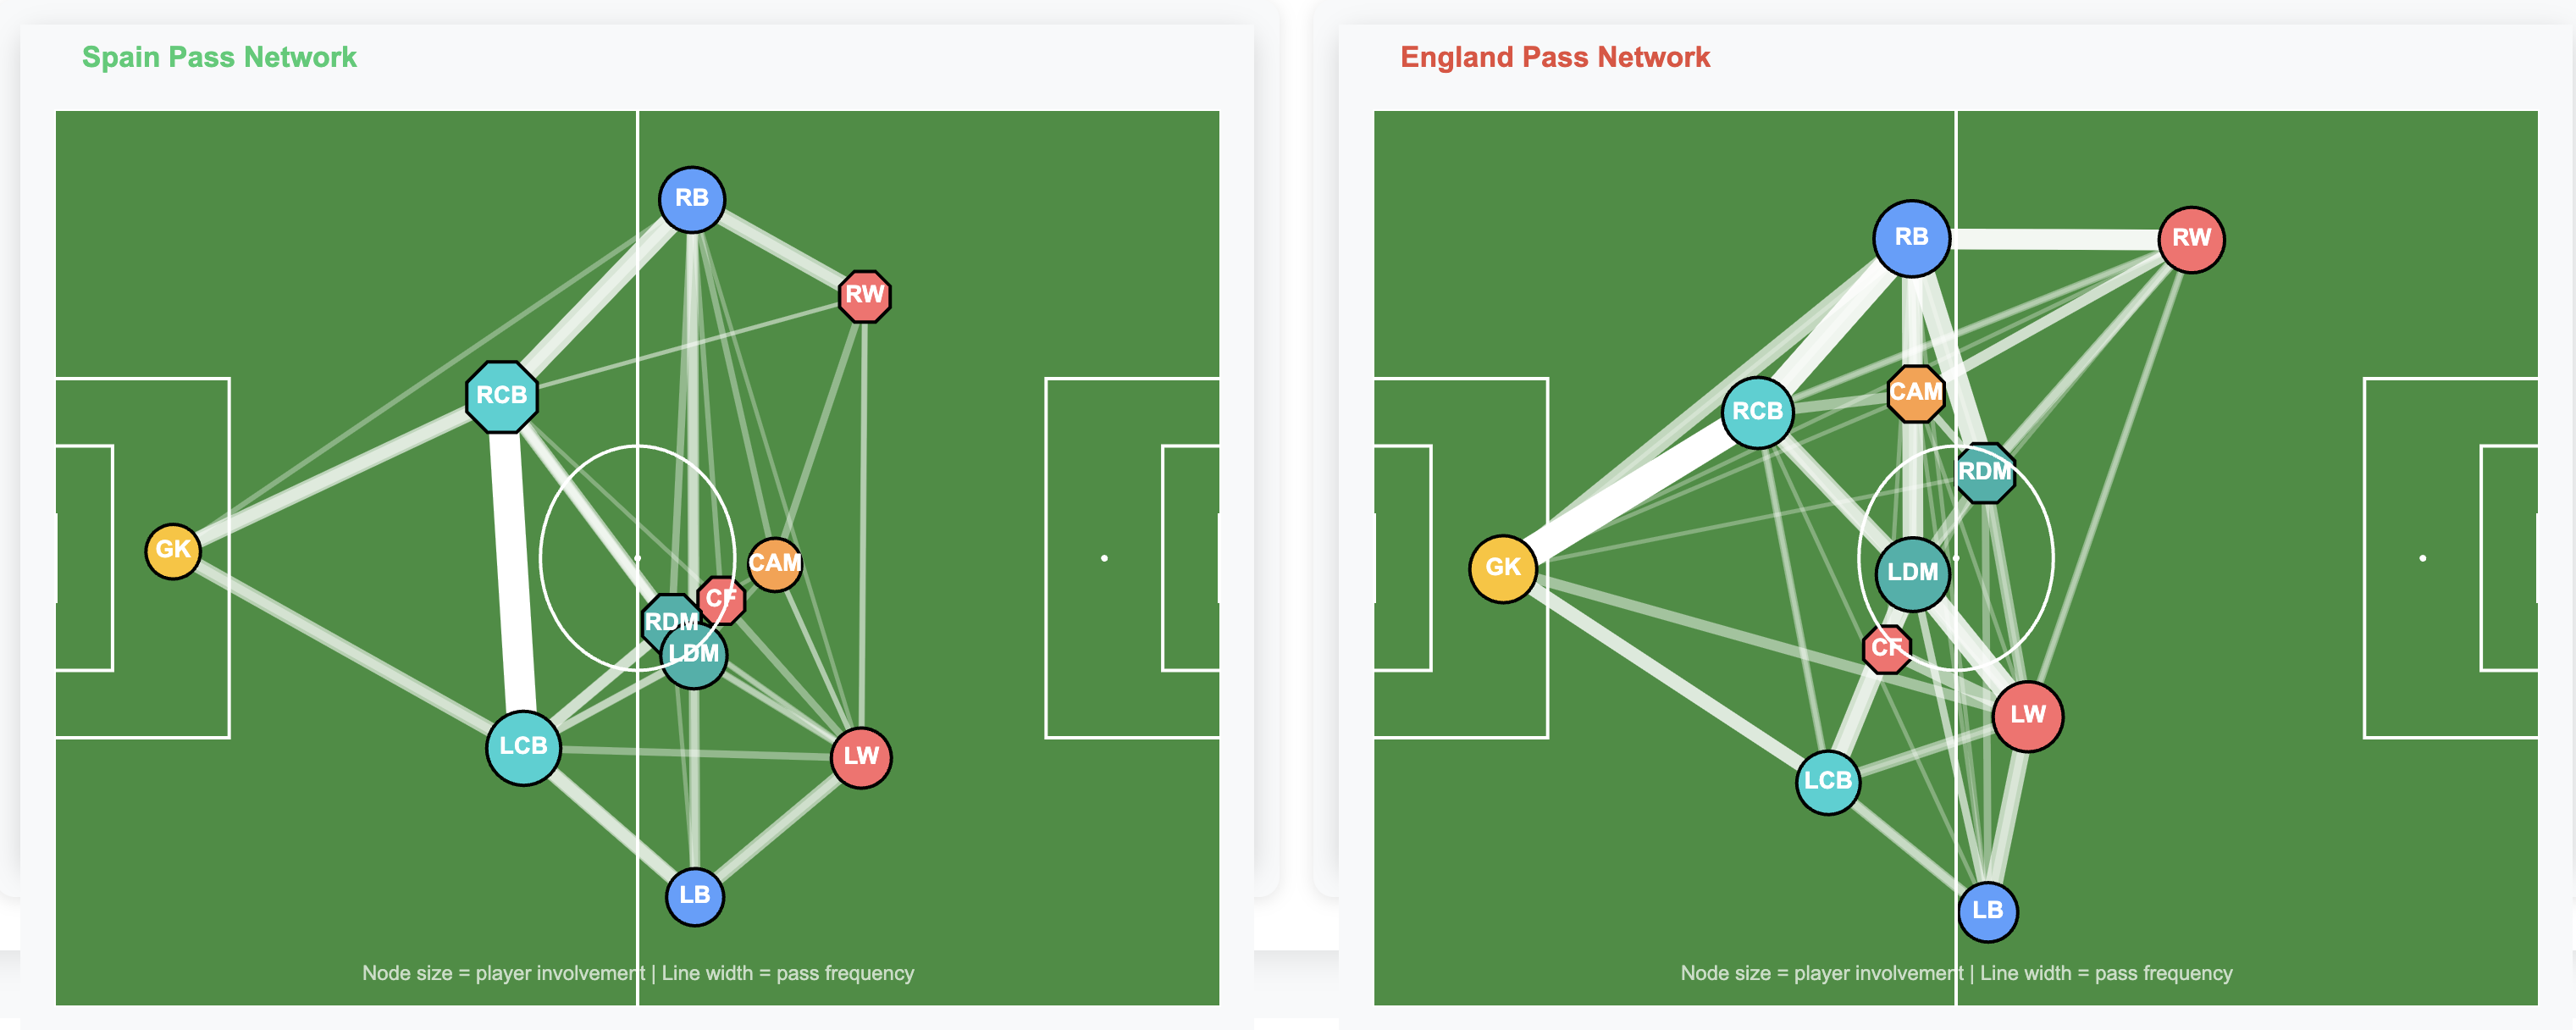
\includegraphics[width=0.9\textwidth]{Spain Eng Pass Network.png}
    \caption{Pass Network Analysis - Force-directed graph layout showing passing relationships between Spain and England players during their UEFA Euro 2024 encounter. Node sizes represent passing involvement, edge thickness indicates pass frequency, and positioning reflects average field positions, as described in Section~\ref{sec:pass_network}.}
    \label{fig:pass_network}
\end{figure}


\begin{figure}[H]
    \centering
    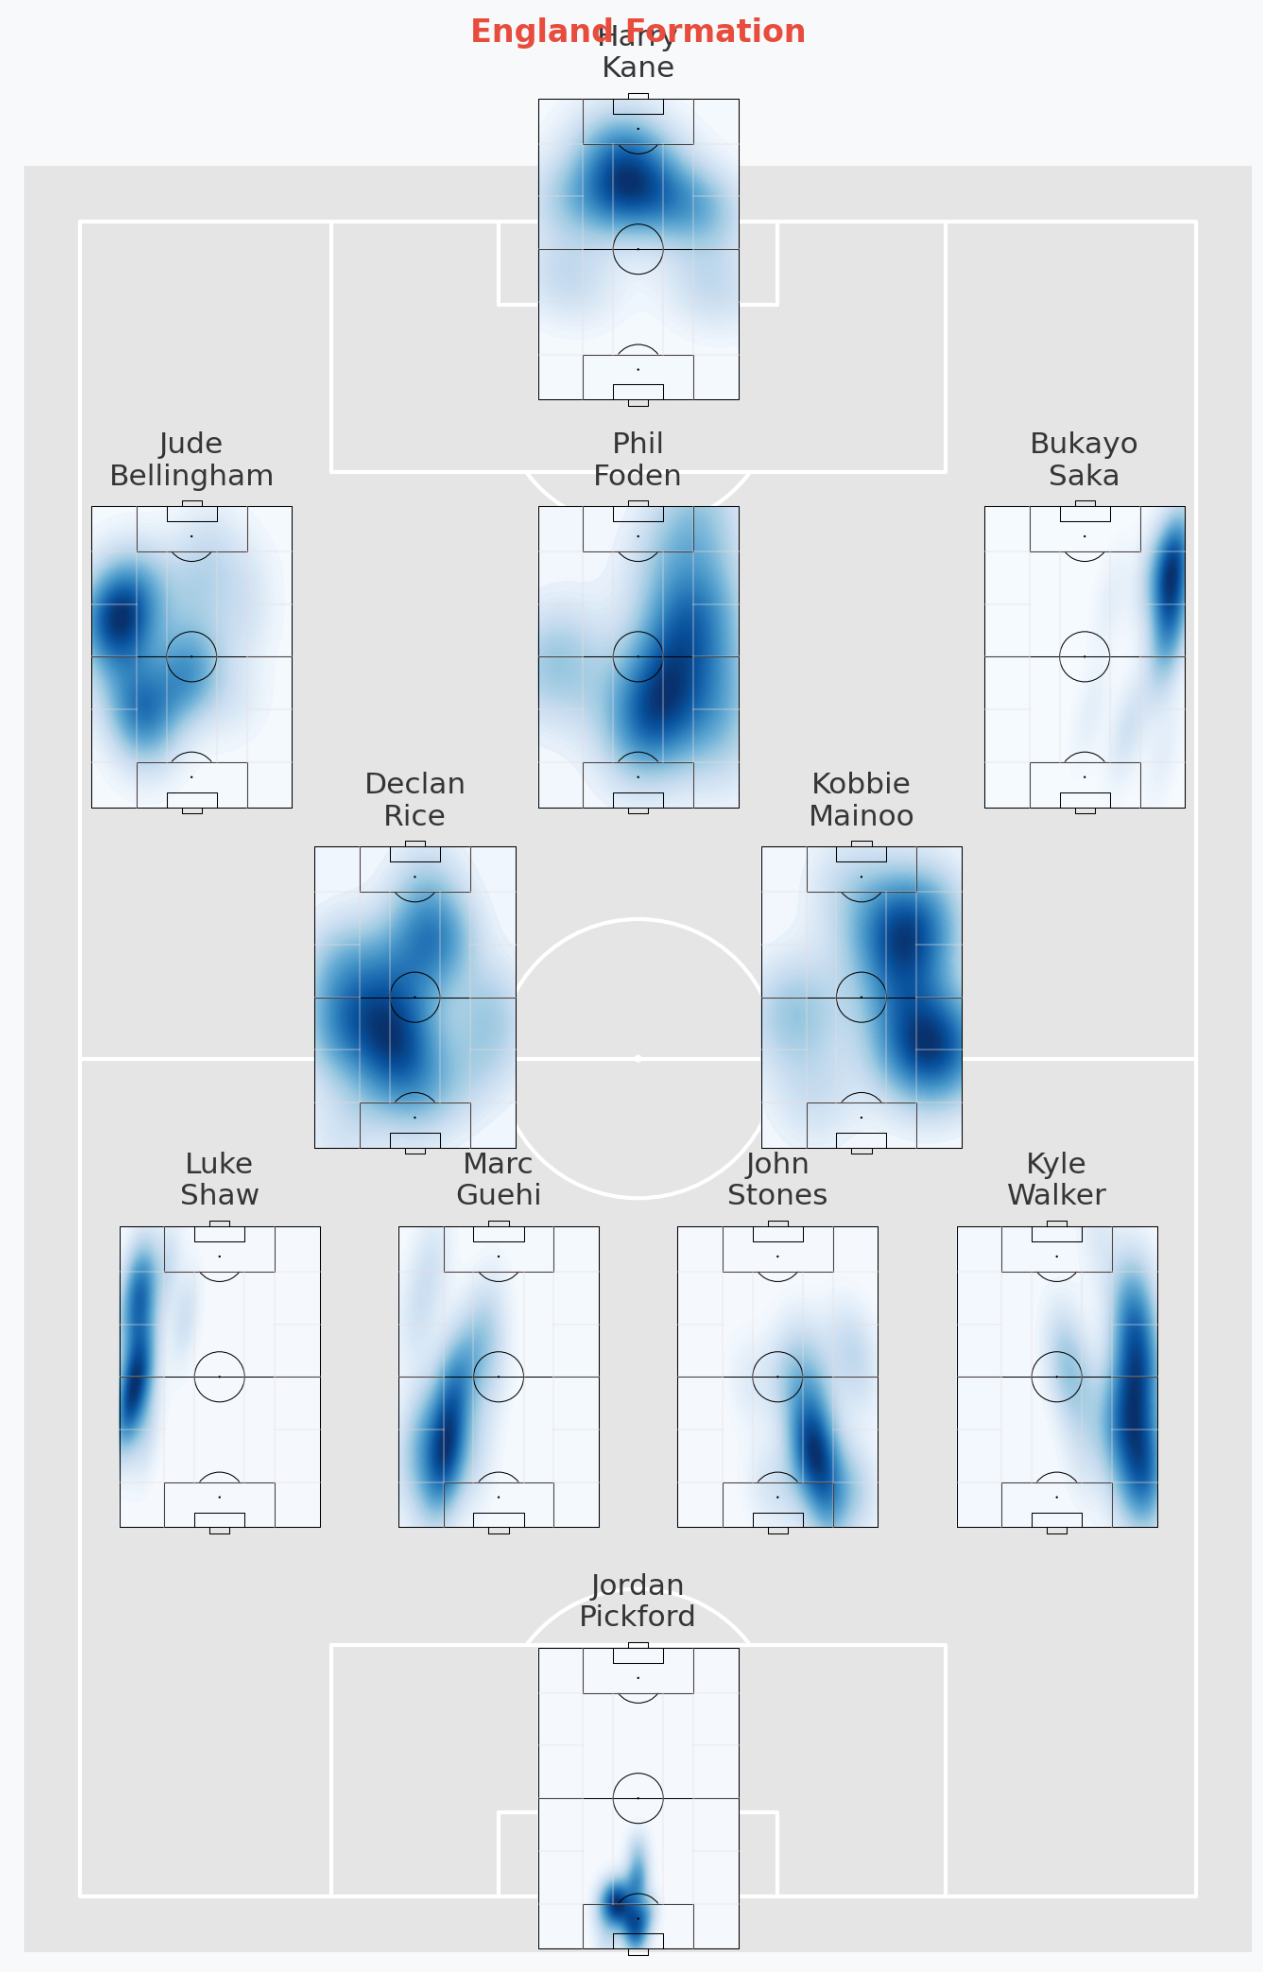
\includegraphics[width=0.85\textwidth,height=0.8\textheight]{Formations.png}
    \caption{Formation Analysis Visualization - Individual player activity density plots arranged in formation grid layout using mplsoccer's formation system. Each subplot shows KDE-based movement patterns derived from Ball Receipt events, with predefined formation-specific offsets preventing positional overlaps, as detailed in Section~\ref{sec:formations_analysis}.}
    \label{fig:formations}
\end{figure}

\subsection{Team Performance Analysis Visualizations}
\begin{figure}[H]
    \centering
    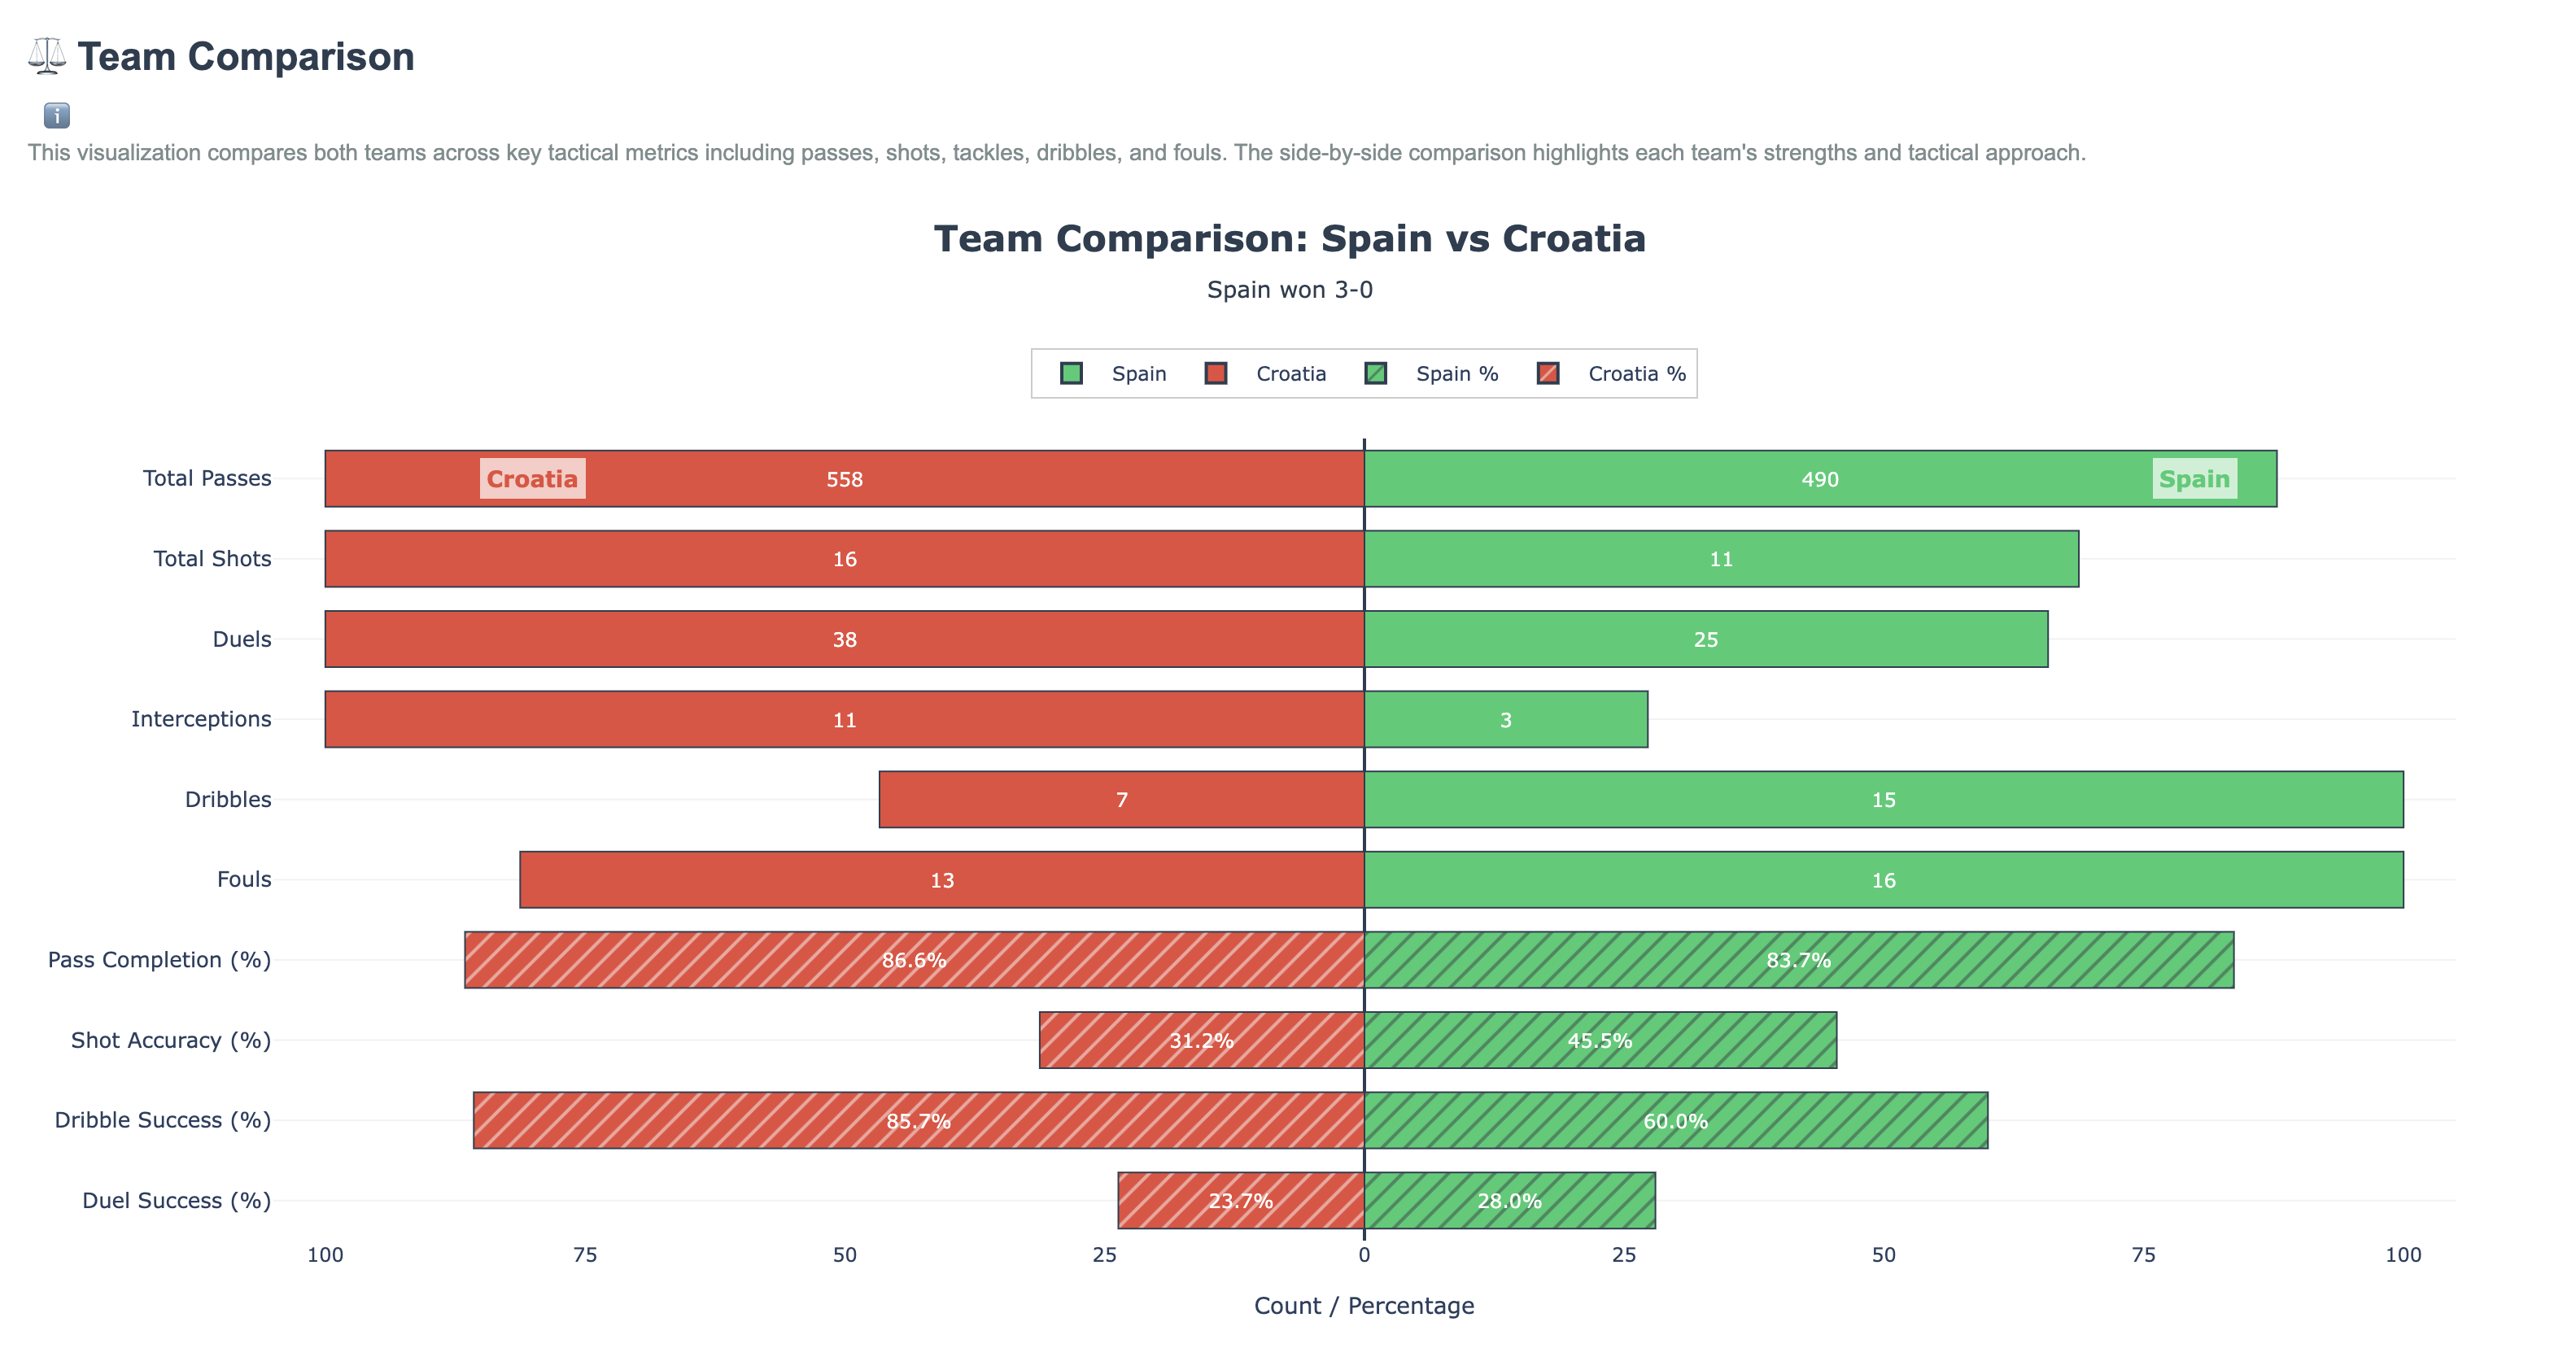
\includegraphics[width=0.9\textwidth]{Team Comparison.png}
    \caption{Team Performance Comparison Dashboard - Comprehensive side-by-side statistical analysis displaying key performance metrics including possession statistics, passing accuracy, shot efficiency, and defensive actions. The symmetric horizontal bar chart layout enables immediate tactical comparison between competing teams, as discussed in Section~\ref{sec:match_statistics}.}
    \label{fig:team_comparison}
\end{figure}
\subsection{Player Performance Visualizations}

\begin{figure}[H]
    \centering
    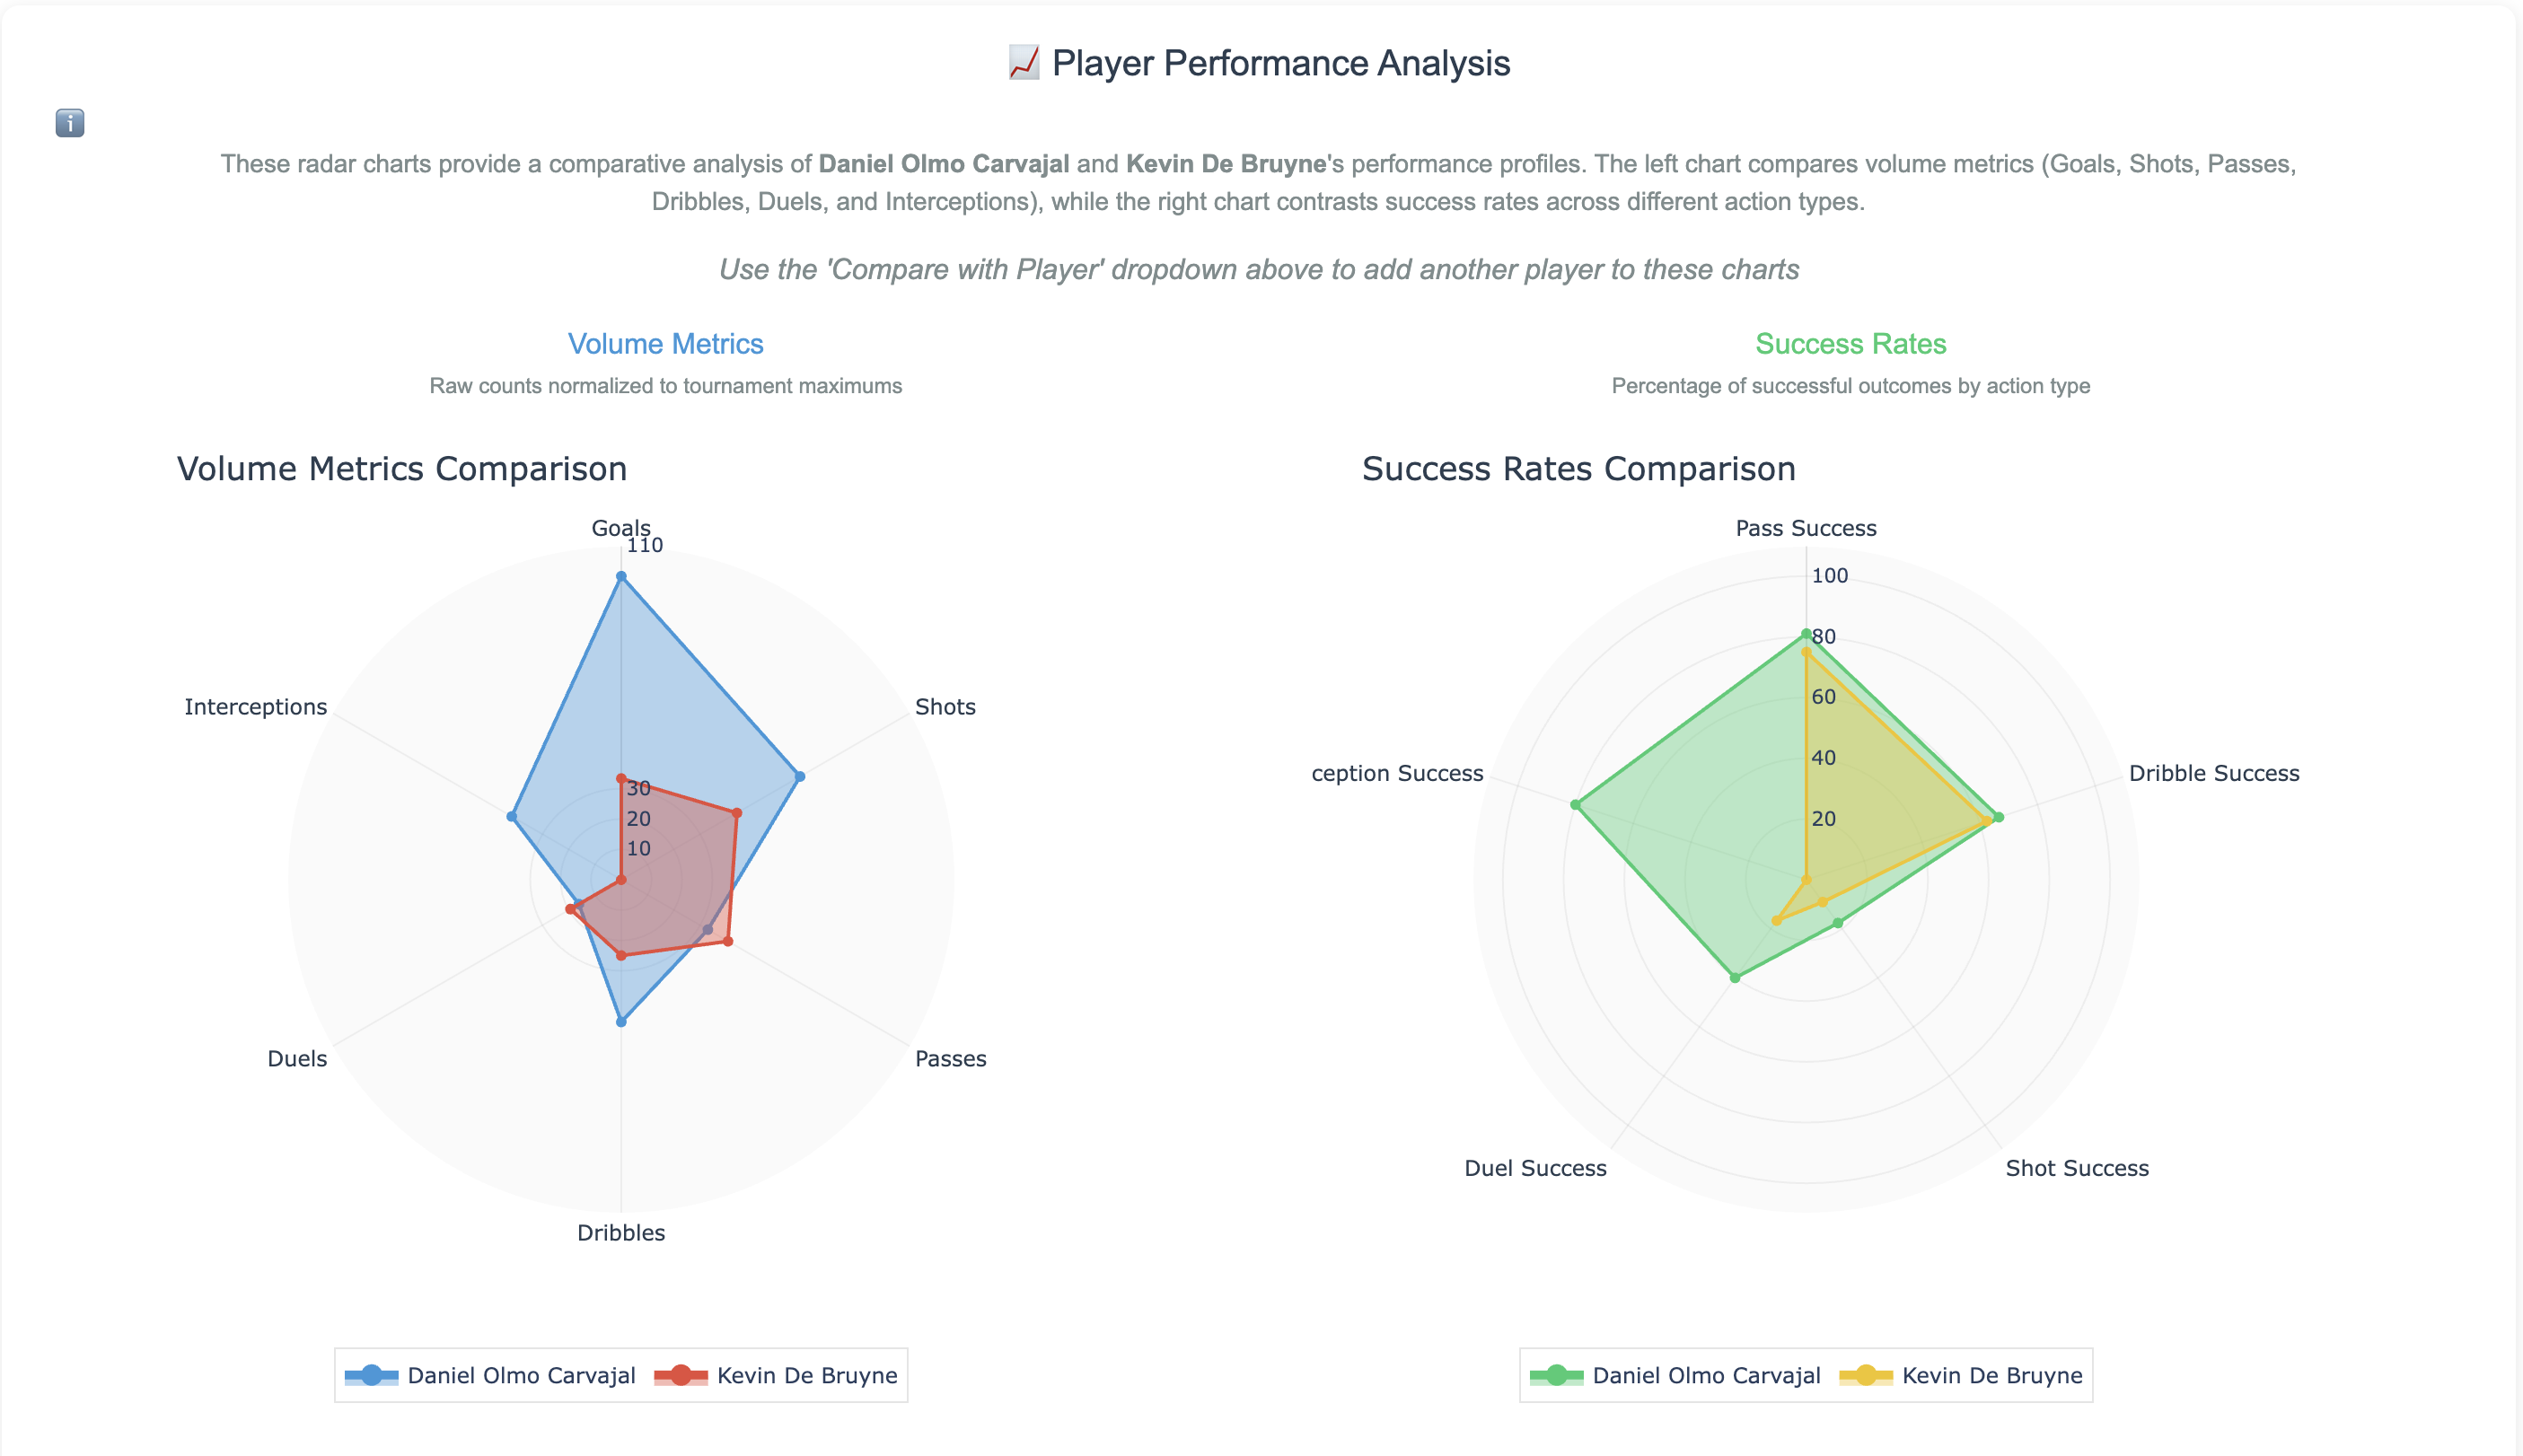
\includegraphics[width=0.9\textwidth]{Player Performance Analysis.png}
    \caption{Individual Player Performance Dashboard - Comprehensive player analysis featuring dual radar charts separating volume metrics (goals, shots, passes, dribbles) from success rate metrics (pass accuracy, shot accuracy, duel success). This innovative visualization approach prevents conflation of activity level with effectiveness, as explained in Section~\ref{sec:performance_metrics}.}
    \label{fig:player_performance}
\end{figure}

\begin{figure}[H]
    \centering
    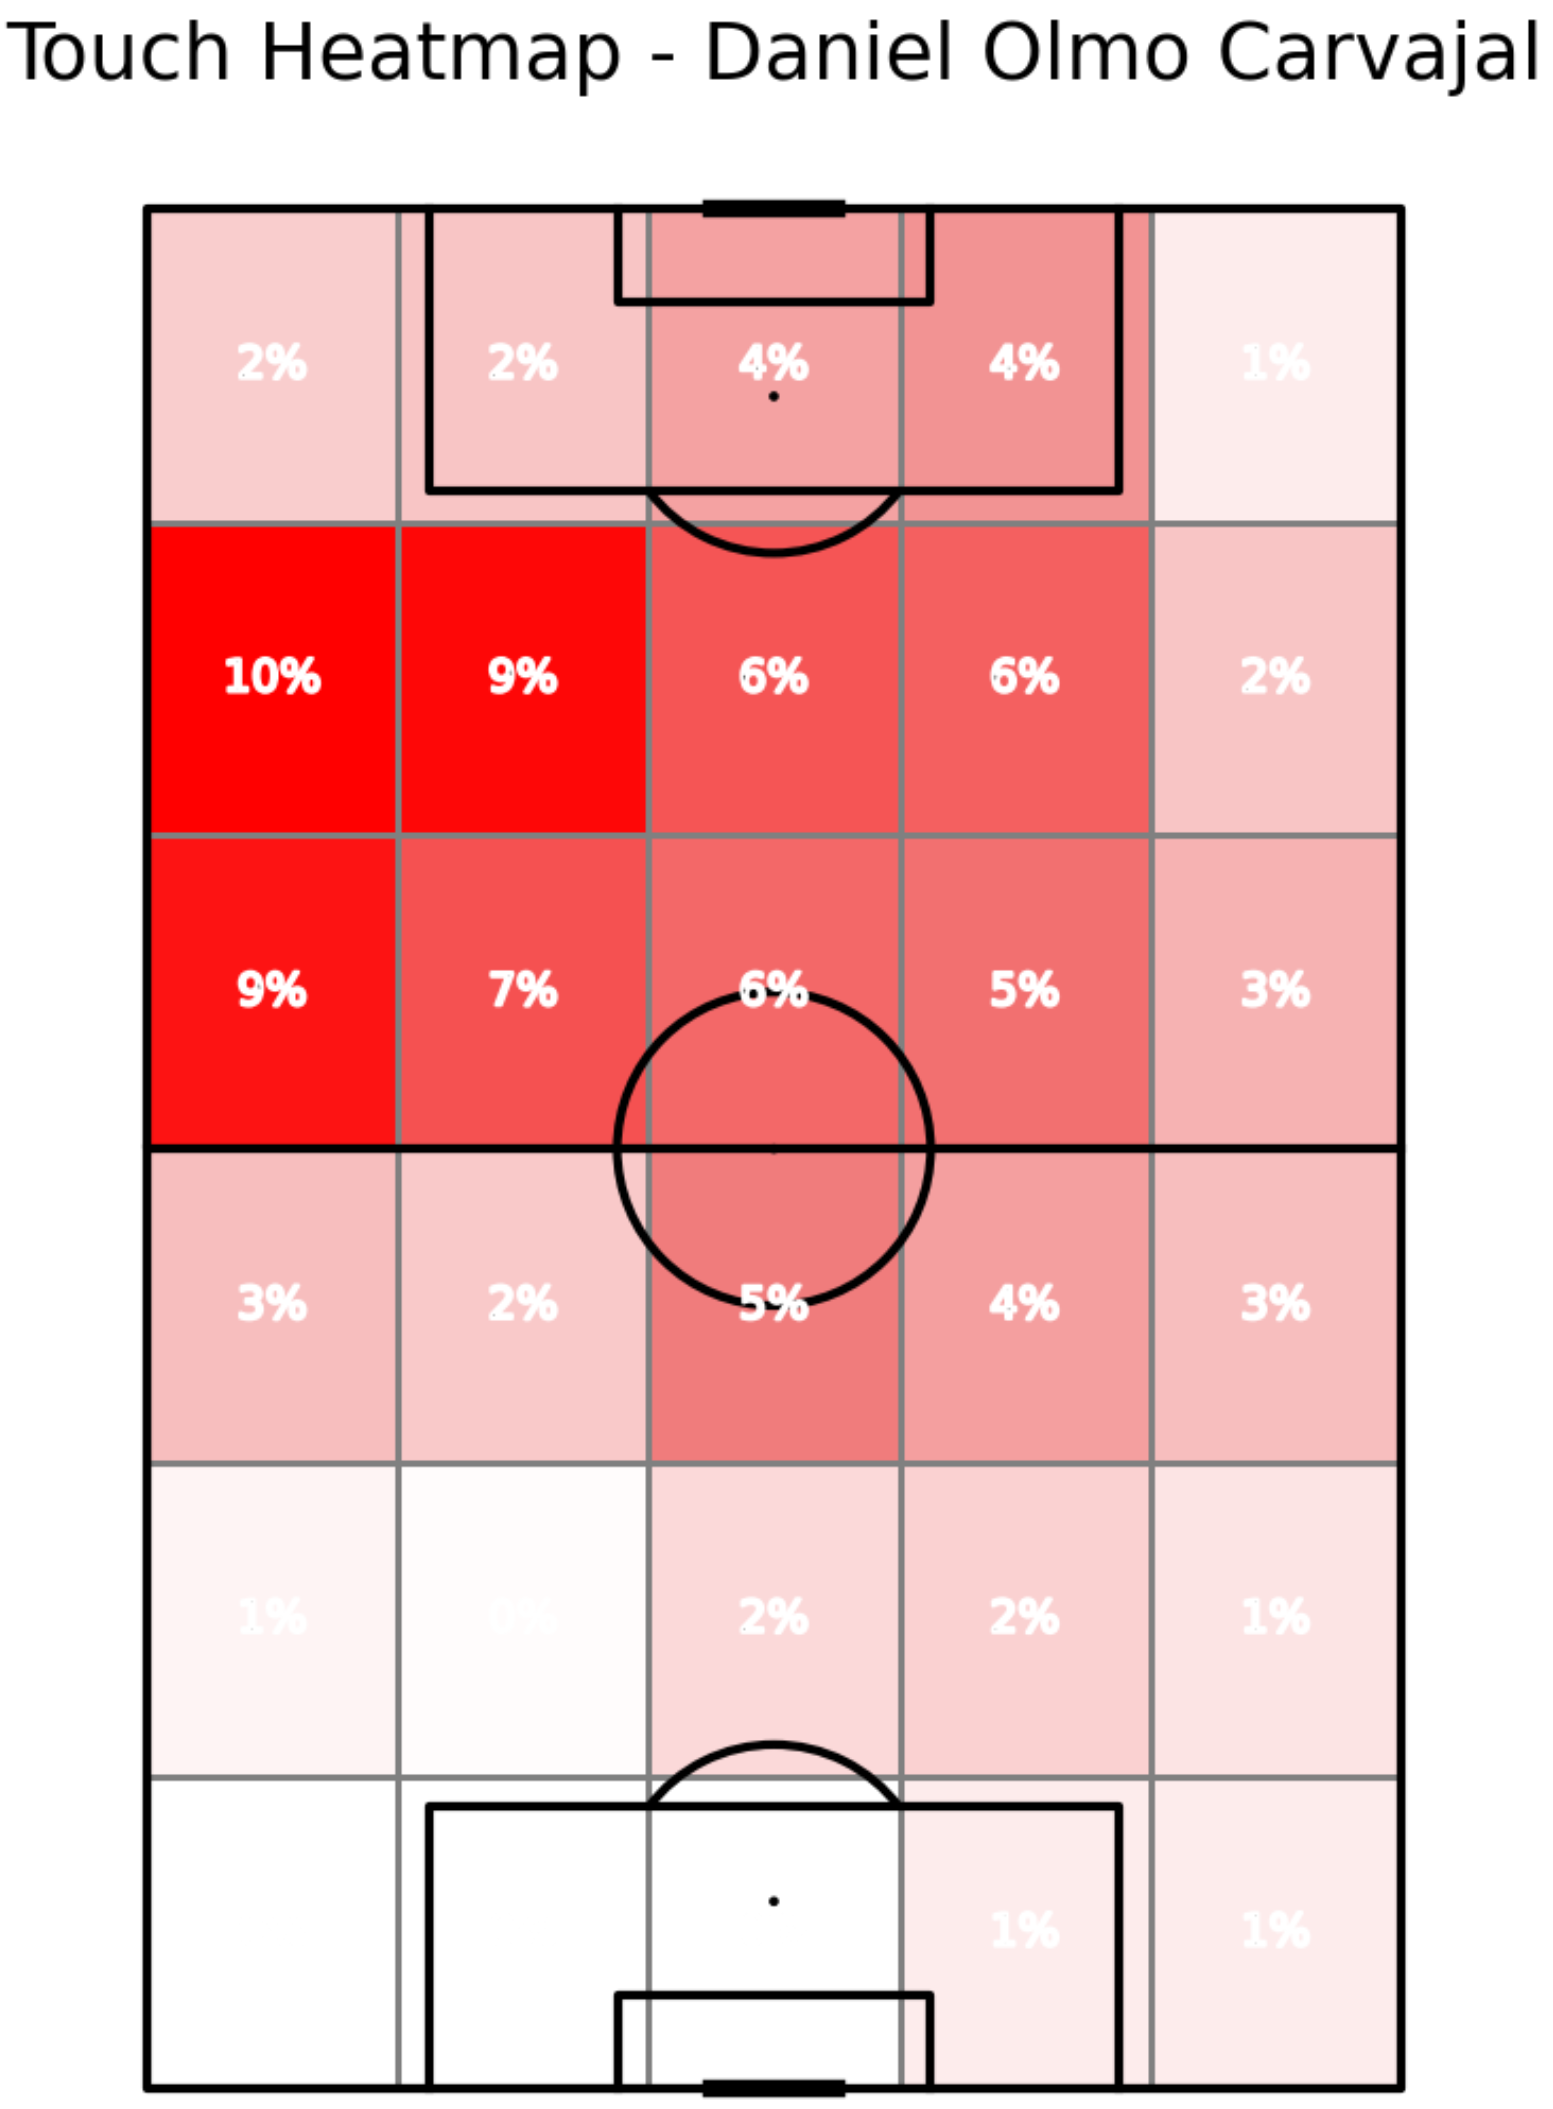
\includegraphics[width=0.85\textwidth]{Touch Heatmap Player.png}
    \caption{Player Touch Heatmap - Grid-based spatial analysis using a 6×5 zone system showing player activity distribution across the football pitch. The percentage-based quantification enables cross-player standardization and comparison, utilizing the methodology outlined in Section~\ref{sec:touch_heatmap}.}
    \label{fig:touch_heatmap}
\end{figure}
\subsection{Event-Level Analysis Visualizations}

\begin{figure}[H]
    \centering
    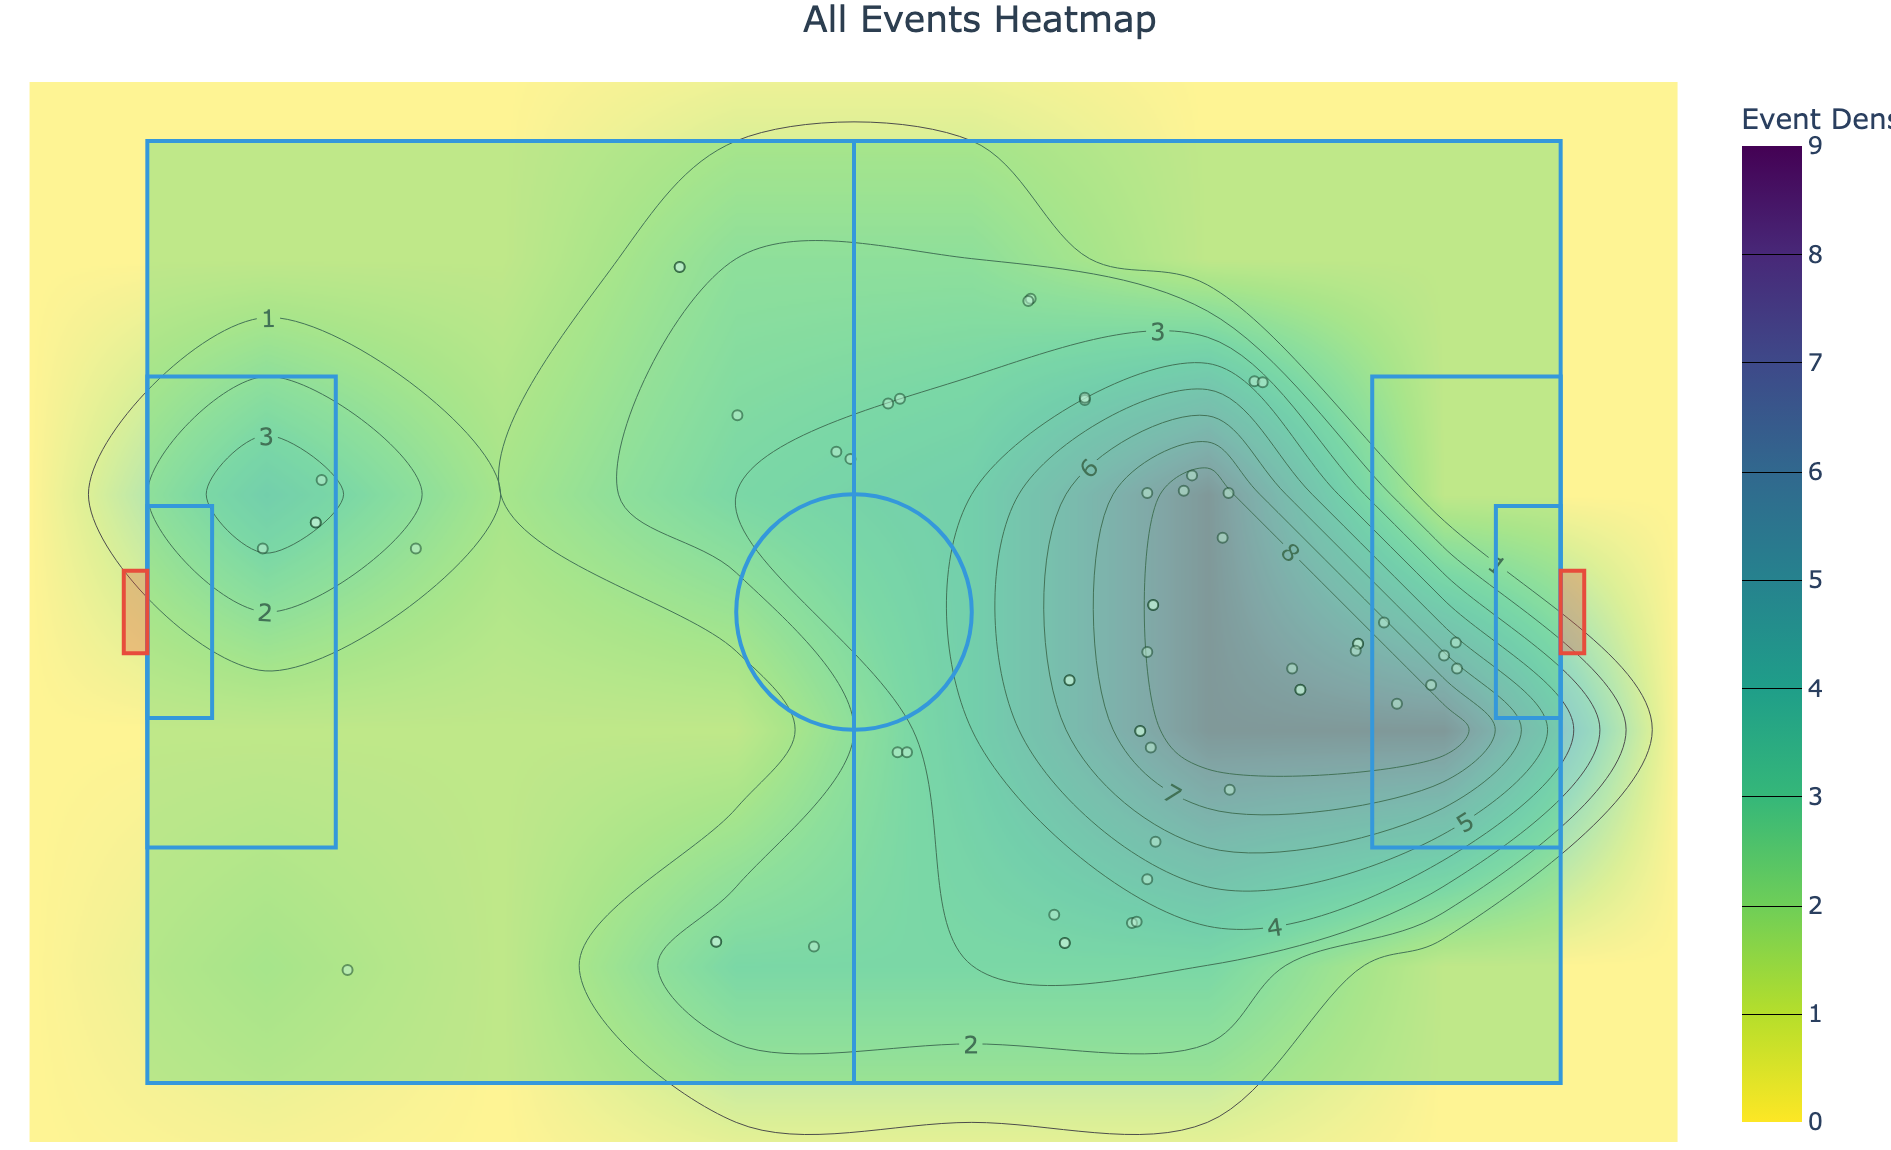
\includegraphics[width=0.9\textwidth]{All Events Heatmap.png}
    \caption{Comprehensive Event Heatmap - Spatial density visualization of all match events plotted on an accurate football pitch representation using mplsoccer coordinates. The color intensity gradient indicates event frequency with darker regions showing higher activity concentration, implementing the spatial analysis framework described in Section~\ref{sec:event_heatmap}.}
    \label{fig:events_heatmap}
\end{figure}

These visualizations collectively demonstrate the dashboard's capability to transform complex football event data into accessible, actionable insights while maintaining analytical rigor and professional visualization standards.

\end{document}
